%!TEX root = Paper.tex

\section{Experiments}
\label{sec:experiments}

\begin{table}[t]
  \centering
  {\small
  \begin{tabular}{rrr|rr} \hline
    $L$ & $K$ & $\Delta$ & $\cascadeucb$ & $\cascadeklucb$ \\ \hline
    16 & 2 & 0.15 & $1290.1 \pm 11.3$ & $357.9 \pm 5.5\phantom{0}$ \\
    16 & 4 & 0.15 & $986.8 \pm 10.8$ & $275.1 \pm 5.8\phantom{0}$ \\
    16 & 8 & 0.15 & $574.8 \pm 7.9\phantom{0}$ & $149.1 \pm 3.2\phantom{0}$ \\
    32 & 2 & 0.15 & $2695.9 \pm 19.8$ & $761.2 \pm 10.4$ \\
    32 & 4 & 0.15 & $2256.8 \pm 12.8$ & $633.2 \pm 7.0\phantom{0}$ \\
    32 & 8 & 0.15 & $1581.0 \pm 20.3$ & $435.4 \pm 5.7\phantom{0}$ \\
    16 & 2 & 0.075 & $2077.0 \pm 32.9$ & $766.0 \pm 18.0$ \\
    16 & 4 & 0.075 & $1520.4 \pm 23.4$ & $538.5 \pm 12.5$ \\
    16 & 8 & 0.075 & $725.4 \pm 12.0$ & $321.0 \pm 16.3$ \\ \hline
  \end{tabular}
  }
  \caption{The $n$-step regret of $\cascadeucb$ and $\cascadeklucb$ in $n = 10^5$ steps. The list $\rnd{A}_t$ is ordered from the largest UCB to the smallest. All results are averaged over $20$ runs.}
  \label{tab:regret bounds}
\end{table}

We conduct four experiments. In \cref{sec:experiments regret bounds}, we validate that the regret of our algorithms scales as suggested by our upper bounds (\cref{sec:upper bounds}). In \cref{sec:experiments worst-first}, we experiment with recommending items $\rnd{A}_t$ in the opposite order, in increasing order of their UCBs. In \cref{sec:experiments imperfect model}, we show that $\cascadeklucb$ performs robustly even when our modeling assumptions are violated. In \cref{sec:experiments ranked bandits}, we compare $\cascadeklucb$ to ranked bandits.


\subsection{Regret Bounds}
\label{sec:experiments regret bounds}

In the first experiment, we validate the qualitative behavior of our upper bounds (\cref{sec:upper bounds}). We experiment with the class of problems $B_\mathrm{LB}(L, K, p, \Delta)$ in \cref{sec:lower bound}. We set $p = 0.2$; and vary $L$, $K$, and $\Delta$. The attraction probability $p$ is set such that it is close to $1 / K$ for the maximum value of $K$ in our experiments. Our upper bounds are reasonably tight in this setting (\cref{sec:discussion}), and we expect the regret of our methods to scale accordingly. We recommend items $\rnd{A}_t$ in decreasing order of their UCBs. This order is motivated by the problem of web search, where higher ranked items are typically more attractive. We run $\cascadeucb$ and $\cascadeklucb$ for $n = 10^5$ steps.

Our results are reported in \cref{tab:regret bounds}. We observe four major trends. First, the regret doubles when the number of items $L$ doubles. Second, the regret decreases when the number of recommended items $K$ increases. These trends are consistent with the fact that our upper bounds are $O(L - K)$. Third, the regret increases when $\Delta$ decreases. Finally, note that $\cascadeklucb$ outperforms $\cascadeucb$. This result is not particularly surprising. $\klucb$ is known to outperform $\ucb$ when the expected payoffs of arms are low \cite{garivier11klucb}, because its confidence intervals get tighter as the Bernoulli parameters get closer to $0$ or $1$.


\subsection{Worst-of-Best First Item Ordering}
\label{sec:experiments worst-first}

\begin{table}[t]
  \centering
  {\small
  \begin{tabular}{rrr|rr} \hline
    $L$ & $K$ & $\Delta$ & $\cascadeucb$ & $\cascadeklucb$ \\ \hline
    16 & 2 & 0.15 & $1160.2 \pm 11.7$ & $333.3 \pm 6.1\phantom{0}$ \\
    16 & 4 & 0.15 & $660.0 \pm 8.3\phantom{0}$ & $209.4 \pm 4.4\phantom{0}$ \\
    16 & 8 & 0.15 & $181.4 \pm 3.9\phantom{0}$ & $60.4 \pm 2.0\phantom{0}$ \\
    32 & 2 & 0.15 & $2471.6 \pm 14.1$ & $716.0 \pm 7.5\phantom{0}$ \\
    32 & 4 & 0.15 & $1615.3 \pm 14.5$ & $482.3 \pm 6.7\phantom{0}$ \\
    32 & 8 & 0.15 & $595.0 \pm 7.8\phantom{0}$ & $201.9 \pm 5.8\phantom{0}$ \\
    16 & 2 & 0.075 & $1989.8 \pm 31.4$ & $785.8 \pm 12.2$ \\
    16 & 4 & 0.075 & $1239.5 \pm 16.2$ & $484.2 \pm 12.5$ \\
    16 & 8 & 0.075 & $336.4 \pm 10.3$ & $139.7 \pm 6.6\phantom{0}$ \\ \hline
  \end{tabular}
  }
  \caption{The $n$-step regret of $\cascadeucb$ and $\cascadeklucb$ in $n = 10^5$ steps. The list $\rnd{A}_t$ is ordered from the smallest UCB to the largest. All results are averaged over $20$ runs.}
  \label{tab:worst-first}
\end{table}

In the second experiment, we recommend items $\rnd{A}_t$ in increasing order of their UCBs. This choice is not very natural and may be even dangerous. In practice, the user could get annoyed if highly ranked items were not attractive. On the other hand, the user would provide a lot of feedback on low quality items, which could speed up learning. We note that the reward in our model does not depend on the order of recommended items (\cref{sec:algorithms}). Therefore, the items can be ordered arbitrarily, perhaps to maximize feedback. In any case, we find it important to study the effect of this counterintuitive ordering, at least to demonstrate the effect of our modeling assumptions.

The experimental setup is the same as in \cref{sec:experiments regret bounds}. Our results are reported in \cref{tab:worst-first}. When compared to \cref{tab:regret bounds}, the regret of $\cascadeucb$ and $\cascadeklucb$ decreases for all settings of $K$, $L$, and $\Delta$; most prominently at large values of $K$. Our current analysis cannot explain this phenomenon and we leave it for future work.


\subsection{Imperfect Model}
\label{sec:experiments imperfect model}

The goal of this experiment is to evaluate $\cascadeklucb$ in the setting where our modeling assumptions are not satisfied, to test its potential beyond our model. We generate data from the \emph{dynamic Bayesian network (DBN) model} of \citet{chapelle09dynamic}, a popular extension of the cascade model which is parameterized by \emph{attraction probabilities} $\rho \in [0, 1]^E$, \emph{satisfaction probabilities} $\nu \in [0, 1]^E$, and the \emph{persistence} of users $\gamma \in (0, 1]$. In the DBN model, the user is recommended a list of $K$ items $A = (a_1, \dots, a_K)$ and examines it from the first recommended item $a_1$ to the last $a_K$. After the user examines item $a_k$, the item attracts the user with probability $\rho(a_k)$. When the user is attracted by the item, the user clicks on it and is satisfied with probability $\nu(a_k)$. If the user is satisfied, the user does not examine the remaining items. In any other case, the user examines item $a_{k + 1}$ with probability $\gamma$. The reward is one if the user is satisfied with the list, and zero otherwise. Note that this is not observed. The regret is defined accordingly. The feedback are clicks of the user. Note that the user can click on multiple items.

The probability that at least one item in $A = (a_1, \dots, a_K)$ is satisfactory is:
\begin{align*}
  \sum_{k = 1}^K \gamma^{k - 1} \bar{w}(a_k) \prod_{i = 1}^{k - 1} (1 - \bar{w}(a_i))\,,
\end{align*}
where $\bar{w}(e) = \rho(e) \nu(e)$ is the probability that item $e$ satisfies the user after being examined. This objective is maximized by the list of $K$ items with largest weights $\bar{w}(e)$ that are ordered in decreasing order of their weights. Note that the order matters.

The above objective is similar to that in cascading bandits (\cref{sec:cascading bandits}). Therefore, it may seem that our learning algorithms (\cref{sec:algorithms}) can also learn the optimal solution to the DBN model. Unfortunately, this is not guaranteed. The reason is that not all clicks of the user are satisfactory. We illustrate this issue on a simple problem. Suppose that the user clicks on multiple items. Then only the last click \emph{can} be satisfactory. But it \emph{does not have to} be. For instance, it could have happened that the user was unsatisfied with the last click, and then scanned the recommended list until the end and left.

We experiment on the class of problems $B_\mathrm{LB}(L, K, p, \Delta)$ in \cref{sec:lower bound} and modify it as follows. The ground set $E$ has $L = 16$ items and $K = 4$. The attraction probability of item $e$ is $\rho(e) = \bar{w}(e)$, where $\bar{w}(e)$ is given in \eqref{eq:attraction probability}. We set $\Delta = 0.15$. The satisfaction probabilities $\nu(e)$ of all items are the same. We experiment with two settings of $\nu(e)$, $1$ and $0.7$; and with two settings of persistence $\gamma$, $1$ and $0.7$. We run $\cascadeklucb$ for $n = 10^5$ steps and use the last click as an indicator that the user is satisfied with the item.

Our results are reported in Figure~\ref{fig:DBN trends}. We observe in all experiments that the regret of $\cascadeklucb$ flattens. This indicates that $\cascadeklucb$ learns the optimal solution to the DBN model. An intuitive explanation for this result is that the exact values of $\bar{w}(e)$ are not needed to perform well. Our current theory does not explain this phenomenon and we leave it for future work.


\subsection{Ranked Bandits}
\label{sec:experiments ranked bandits}

\begin{figure}[t]
  \centering
  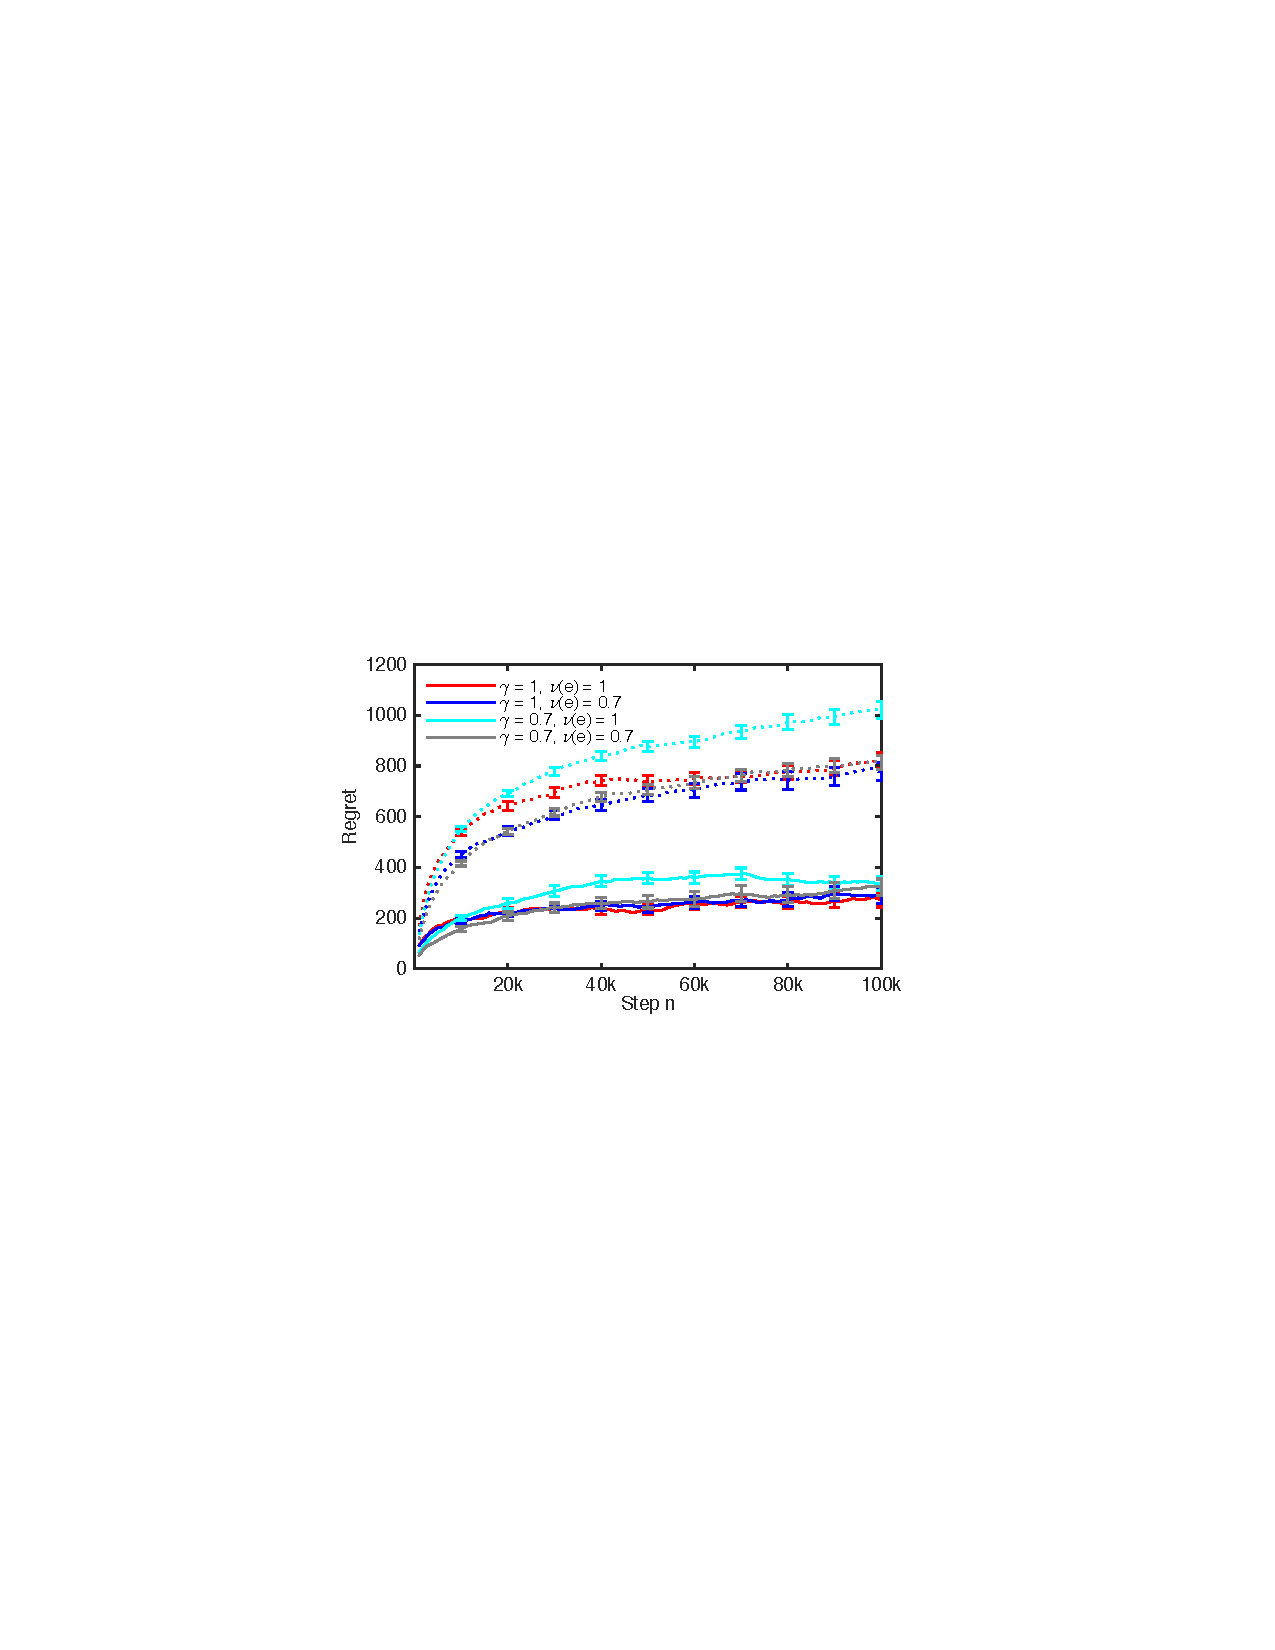
\includegraphics[width=3.2in, bb=2.15in 4.25in 6.15in 6.75in]{Figures/DBNTrends}
  \caption{The $n$-step regret of $\cascadeklucb$ (solid lines) and $\rankedklucb$ (dotted lines) in the DBN model in \cref{sec:experiments imperfect model}.}
  \label{fig:DBN trends}
\end{figure}

In our final experiment, we compare $\cascadeklucb$ to a ranked bandit (\cref{sec:related work}) where the base bandit algorithm is $\klucb$. We refer to this method as $\rankedklucb$. The choice of the base algorithm is motivated by the following reasons. First, $\klucb$ is the best performing oracle in our experiments. Second, since both compared approaches use the same oracle, the difference in their regrets is likely due to their statistical efficiency, and not the oracle itself.

The experimental setup is the same as in \cref{sec:experiments imperfect model}. Our results are reported in Figure~\ref{fig:DBN trends}. We observe that the regret of $\rankedklucb$ is significantly larger than the regret of $\cascadeklucb$, about three times. The reason is that the regret in ranked bandits is $\Omega(K)$ (\cref{sec:related work}) and $K = 4$ in this experiment. The regret of our algorithms is $O(L - K)$ (\cref{sec:discussion}). Note that $\cascadeklucb$ is not guaranteed to be optimal in this experiment. Therefore, our results are encouraging and show that $\cascadeklucb$ could be a viable alternative to more established approaches.
